\chapter{Morphisms of (pre)sheaves, Yoneda lemma, étalé space}

\remyquote{You can do what you want, it's a free world (on one generator).}
%% NOTE: You can do what you want [with respect to underlining/boldfacing names of categories]

\section{Morphisms of (pre)sheaves}

\begin{defn}
Let $\cat C$ be a small category.
Then \indexdefn{$\catPresheaf(\cat C)$} is the functor category $\catFunctor(\cat C\opp,\catSet)$: its objects are functors $F\colon\cat C\opp\to\catSet$, and its morphisms $\alpha\colon F\To G$ are \emph{natural transformations}\index{natural transformation}, that is, collections of functions $\alpha_X\colon F(X)\to G(X)$ for all $X\in\cat C$ such that the diagram
\begin{equation*}
    \begin{tikzcd}
        F(Y) \ar[r, "\alpha_Y"] \ar[d, "F(f)"'] & G(Y) \ar[d, "G(f)"] \\
        F(X) \ar[r, "\alpha_X"'] & G(X)
    \end{tikzcd}
\end{equation*}
commutes for all $f\colon X\to Y$ in $\cat C$.
\end{defn}

\begin{defn}
Let $X$ be a topological space.
Then the category of presheaves on $X$ is $\catPresheaf(X)\coloneqq\catPresheaf(\open(X))$\index{$\catPresheaf(X)$} and the category of sheaves on $X$ is the full subcategory $\catSheaf(X)\subseteq\catPresheaf(X)$\index{$\catSheaf(X)$} on the sheaves.
\end{defn}

\begin{lem}\label{lem:psh-category-set}
Let $\cat C$ be a small category.
Then:
\begin{enumerate}
\item $\catPresheaf(\cat C)$ is a category.
\item The category $\catPresheaf(\cat C)$ has all (small) limits\index{limit} and colimits\index{colimit}, and they are computed objectwise; e.g., for presheaves $F,G\in\catPresheaf(\cat C)$ the natural map
    \[ (F\times G)(U) \to F(U)\times G(U) \]
    is an isomorphism for all open $U\subseteq X$.
\item A natural transformation $\alpha\colon F\To G$ between presheaves $F$ and $G$ on $\cat C$ is invertible if and only if the component $\alpha_X\colon F(X)\to G(X)$ is a bijection for all $X\in\cat C$.
\end{enumerate}
\end{lem}

\begin{rmk}
Colimits\index{colimit} in the category $\catSheaf(X)$ of sheaves will be more complicated.
\end{rmk}

\begin{exmp}
Recall that we defined a sheaf $h_Z$ on $X$ for $Z\in\catTopologicalSpace$ (\cref{exmp:ct-maps-presheaf}).
If $g\colon Z\to Z'$ is a continuous map, then we get a natural transformation $h_Z\To h_{Z'}$ with component
\[ \cont(U,Z) \to \cont(U,Z')\text{,} \quad f \mapsto g\circ f \]
at $U\in\open(X)$.
One checks that this is natural.
\end{exmp}

\begin{exmp}
For the sheaf of sections (\cref{exmp:sheaf-of-sections}), a map $g\colon Y\to Y'$ over $X$ induces a natural transformation $h_{Y/X}\To h_{Y'/X}$ with component
\[ \cont[X](U,Y) \to \cont[X](U,Y')\text{,} \quad s \mapsto g\circ s \]
at $U\in\open(X)$.
This is again natural in $U$.
\end{exmp}

In fact, the sheaf $h_Z$ is a special case of $h_{Y/X}$:
\begin{lem}
If $Y=Z\times X\xrightarrow{\pr_X} X$ in $\catTopologicalSpace_{/X}$, then the sheaves $h_{Y/X}$ and $h_Z$ are isomorphic.
\end{lem}
\todo{Picture}
\begin{proof}
For $U\in\open(X)$, define
\[ \cont[X](U,Z\times X) \to \cont(U,Z)\text{,} \quad s\mapsto \pr*_Z\circ s \]
and
\[ \cont(U,Z) \to \cont[X](U,Z\times X)\text{,} \quad f \mapsto (u\mapsto (f(u),u))\text{.} \]
These maps are inverses.
Both transformations are natural. For the first: given an inclusion of opens $U\subseteq V\subseteq X$, the diagram
\begin{equation*}
    \begin{tikzcd}
        \cont[X](V,Z\times X) \ar[r, "\pr*_Z\circ -"] \ar[d, "(-)|_U"'] & \cont(V,Z) \ar[d, "(-)|_U"] \\
        \cont[X](U,Z\times X) \ar[r, "\pr*_Z\circ -"'] & \cont(U,Z)
    \end{tikzcd}
\end{equation*}
commutes.
\end{proof}

\begin{exmp}
Let $Y\to X$ be the two-to-one cover $\sphere[1]\to\sphere[1]$\index{circle covering}.
Then $h_{Y/X}$ is not isomorphic to $h_Z$ for any $Z\in\catTopologicalSpace$ (but it is locally isomorphic to $h_{\{1,2\}}$, as we will see later\todo{Ref back}).

Suppose $h_{Y/X}\cong h_Z$ for $Z\in\catTopologicalSpace$.
Then $Z\neq\emptyset$, for
\[ h_\emptyset(U) = \begin{cases}
    \emptyset & \text{if } U \neq\emptyset\text{,} \\
    \terminal & \text{if } U =\emptyset\text{.}
\end{cases} \]
But we have seen that $h_{Y/X}$ is nonempty for a small enough interval.
So $Z\neq\emptyset$, so constant maps show that $h_Z(U)\neq\emptyset$ for all $U$.
But last lecture, we saw that $h_{Y/X}(X)=\emptyset$.
\todo{Ref}
\end{exmp}

\section{Yoneda lemma}

\begin{defn}
Let $\cat C$ be a small category.
Then the \emph{representable presheaf}\index{presheaf!representable} on $X\in\cat C$ is the presheaf
\[ h_X \colon \cat C\opp\to\catSet\text{,} \quad Y \mapsto \Hom[\cat C](Y,X) \]
with restriction map
\[ f^*\colon\Hom[\cat C](X,Y')\to\Hom[\cat C](X,Y)\text{,} \quad g\mapsto g\circ f\text{.} \]
induced by $f\colon Y\to Y'$ in $\cat C$.
\end{defn}

\begin{rmk}
The sheaf $h_Z$ on $X$ from \cref{exmp:ct-maps-presheaf} is \emph{not} a representable presheaf on $\open(X)$.
The sheaf $h_Z$ sends an open $U\subseteq X$ to the set $\cont(U,Z)$ of all continuous  maps $U\to Z$, whereas the representable presheaf $h_V$ represented by an open $V\subseteq X$ sends $U\subseteq X$ to the set $\Hom[\open(X)](U,V)$ of inclusions $U\hookrightarrow V$ (a subsingleton set).
The sheaf $h_Z$ can be regarded as the \emph{restriction} of the representable presheaf $h_Z = \Hom[\catTopologicalSpace](-,Z)$ on the (non-small) category of spaces to the (non-full) subcategory $\open(X)\subseteq\catTopologicalSpace$.
\end{rmk}

In some sense, the representable presheaf represented by $X$ is `freely generated' by the section $\id_X\in h_X(X)$.

\begin{lem}[name={\indexdefn{Yoneda lemma}~\cite[Theorem~2.2.4]{riehlCategoryTheoryContext2016}}]\label{lem:yoneda}
    Let $F: \cat C\opp \to \catSet$ be a functor, $X \in \cat C$. Then the map \[
    \Phi: \Hom_{\catPresheaf(\cat C)}(h_X, F) \to F(X)\text{,} \quad \alpha\mapsto \alpha_X(\id_X)
    \] is a bijection that is natural in $F$ and $X$. 
\end{lem}
\begin{proof}
    We leave the naturality in $F$ and $X$ as an exercise. Part of the exercise is to work out what is meant by naturality in $F$ and $X$. \todo{maybe add details}
    The inverse of $\Phi$ will be a map \[
    \Psi: F(X) \to \Hom_{\catPresheaf(C)}(h_X, F)
    \] defined by $s \mapsto (f \mapsto F(f)(s))_{Y \in \cat C}$.
    The first thing to check is that this map lands in $\Hom_{\catPresheaf(\cat C)}(h_X, F)$. That is, we need to check $\Psi(s)$ is a natural transformation. This is true: given $g: Y \to Z$ in $\cat C$ the diagram 
    \[
    \begin{tikzcd}
{\Hom(Z,X)} \arrow[d, "-\circ g"'] \arrow[r, "\Psi(s)_Z"] & F(Z) \arrow[d, "F(g)"] \\
{\Hom(Y,X)} \arrow[r, "\Psi(s)_Y"']                       & F(Y)            
\end{tikzcd}
    \] commutes, since we have $F(g)(\Psi(s)_Z(f)) = F(g)(F(f)(s)) = F(fg)(s) = \Psi(s)_Y(fg)$.
    We check that $\Psi$ provides an inverse for $\Phi$. One side is immediate: $\Phi \Psi(s) = \Psi(s)_X(\id_X) = F(\id_X)(s) = s$. 
    For the converse, let $\alpha: h_X \to F$ be a natural transformation. We check that $\Psi \Phi(\alpha) = \alpha$. 
    Let $Y \in \cat C$, and $f \in \Hom(Y, X)$. The naturality of $\alpha$ gives a commutative diagram
    \[
    \begin{tikzcd}
{\Hom(X,X)} \arrow[d, "-\circ f"'] \arrow[r, "\alpha_X"] & F(X) \arrow[d, "F(f)"] \\
{\Hom(Y,X)} \arrow[r, "\alpha_Y"']                        & F(Y)                  
\end{tikzcd}
\] We now have $\Psi(\Phi \alpha)_Y(f) = F(f)(\Phi \alpha) = F(f) (\alpha_X(\id_X)) = \alpha_Y (\id_X \circ f)= \alpha_Y(f)$ by plugging in $\id_X$ into the diagram above. 
\end{proof}

\section{Étalé space}

In the coming lectures, we will show that every sheaf on a space $X$ is isomorphic to $h_{Y/X}$ for some map $Y\to X$.
We will construct a functor $\etalespace*\colon\catPresheaf(X)\to\catTopologicalSpace_{/X}$ which sends a presheaf to its \emph{étalé space} (also called \emph{espace étalé}\index{espace étalé|see{étalé space}}, (wrongly) \emph{étale space} or \emph{sheaf space} (but we do not like that)).

The idea is as follows: a presheaf $F$ is determined by its values $F(U)$ for opens $U\subseteq X$ and the restriction maps.
By the Yoneda lemma, the values can be written as $F(U)\cong\Hom[\catPresheaf(X)](h_U,F)$.
For $h_U$, the étalé space will be the space $U\to X$ over $X$.
In general, a presheaf $F$ is `generated by copies of $h_U$ modulo relations from the restrictions'.
We define $\etalespace(F)\to X$ by glueing copies of $U$ `along the same colimit diagram' (but now in $\catTopologicalSpace_{/X}$ instead of $\catPresheaf(X)$).

\begin{defn}\label{defn:espace-étalé}
Let $F$ be a presheaf on $X$.
The \indexdefnemph{étalé space} $\etalespace(F)$ is the quotient of the coproduct
\[ \coprod_{U\in\open(X)} F(U)\times U \]
(where $F(U)$ is endowed with the discrete topology), with notation $(s,x)_U$ for the point given by $s\in F(U)$ and $x\in U$ in the factor indexed by $U$, by the equivalence relation generated by
\[ (s|_U, x)_U \sim (s, x)_V \]
for $(s,x)\in F(V)\times U$ for $x\in U\subseteq V$.
\end{defn}

Categorically, the étalé space is the \indexterm{coequaliser}
\[ \etalespace(F) = \coeq\bigl(\coprod_{U\subseteq V\subseteq X} F(V)\times U \rightrightarrows \coprod_{U\subseteq X} F(U)\times U\bigr)\]
where the arrows are given by
\begin{equation*}
    \begin{tikzcd}[row sep=tiny]
        F(U)\times U & F(V)\times U \ar[l, "\incl*^*\times\id"'] \ar[r, "\id\times \incl*"] & F(V)\times V \\
        (s|_U, x) \ar[u, "\in", phantom, marking] & (s,x) \ar[l, mapsto] \ar[r, mapsto] \ar[u, "\in", phantom, marking] & (s,x) \ar[u, "\in", phantom, marking]
    \end{tikzcd}
\end{equation*}
where $\incl*\colon U\hookrightarrow V$ denotes the inclusion map.

Alternatively, the étalé space $\etalespace(F)$ is the \indexterm{coend}
\[ \etalespace(F) = \int^{U\in\open(X)} F(U)\times U\text{.} \]

To understand the étalé space a bit better, we have to understand the equivalence relation generated by the given relation, with respect to which we take the quotient.

\begin{rmk}\label{rmk:equivalence-relation-generated}
Let $\sim$ be a relation on a set $X$.
The equivalence relation $\approx$ on $X$ generated by $\sim$ can be explicitly defined as follows: we say $x\approx y$ if and only if there is a finite zigzag
\begin{equation*}
    \begin{tikzcd}
        & a_1 & & a_3 & & a_{2n-1} \\
        x = a_0 \ar[ru, "\sim"] & & a_2 \ar[lu, "\sim"'] \ar[ru, "\sim"] & & \ldots \ar[lu, "\sim"'] \ar[ru, "\sim"] & & a_{2n}=y \ar[lu, "\sim"']
    \end{tikzcd}
\end{equation*}
of elements $a_i\in X$ such that $x=a_0$, $y=a_{2n}$, $a_{2i}\sim a_{2i+1}$ for $0\leq i<n$ and $a_{2i}\sim a_{2i-1}$ for $0<i\leq n$.
\end{rmk}

\begin{exmp}
To compute the \indexterm{coequaliser} of the diagram of sets
\begin{equation*}
    \begin{tikzcd}
        \{1,2\} \ar[r, shift left, "-\cdot 1"] \ar[r, shift right, "-\cdot 2"'] & \{1,2,3,4\}
    \end{tikzcd}
\end{equation*}
where the maps multiply by one and two, respectively, we need to understand the equivalence relation generated by $x\sim 2x$ for all $x\in\{1,2\}$.
That is, we have $1\sim 2$ and $2\sim 4$, and nothing more.
The equivalence classes in the relation $\approx$ generated by $\sim$ then are $\{1,2,4\}$ and $\{3\}$.
\end{exmp}

\begin{lem}
If $(s,x)_U\in F(U)\times U$ and $(t,y)_V\in F(V)\times V$, then $(s,x)_U\approx (t,y)_V$ (that is, they are equivalent under the equivalence relation generated by $\sim$ as in \cref{defn:espace-étalé}) if and only if $x = y$ and there exists an open neighbourhood $W\subseteq U\cap V$ of $x$ such that $s|_W = t|_W$.
\end{lem}

One can prove this lemma using the explicit description of $\approx$ given in \cref{rmk:equivalence-relation-generated}, but this is difficult combinatorics!
A better proof shows that the relation on the right in the equivalence of the lemma is an equivalence relation and that the former statement implies the latter (i.e., `$\sim$ implies $\approx$').

\begin{exmp}\label{exmp:representable-presheaf-espace-étalé}
If $F = h_U$ is the representable presheaf\index{presheaf!representable} on $X$ represented by an open $U\subseteq X$ (see \cref{fig:presheaf-represented-by-U}), then
\[ F(V) = \Hom[\open(X)](V,U) = \begin{cases}
    \terminal & \text{if } V\subseteq U\text{,} \\
    \emptyset & \text{if } V\not\subseteq U\text{.}
\end{cases}\]
The étalé space $\etalespace(F)$ is the quotient of
\[ \coprod_{V\subseteq X} F(V)\times V = \coprod_{V\subseteq U} V \]
by the equivalence relation generated by $(*,x)_V\sim(*,x)_{V'}$ for all $V,V'\subseteq U$.
This just leaves $U$, so $\etalespace(h_U) = U$.
\end{exmp}

\begin{figure}
    \centering
    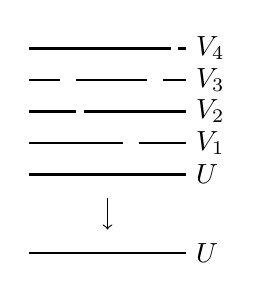
\begin{tikzpicture}
        \node (U) at (2, 0) [right] {\(U\)};
        \node (U') at (2, 1) [right] {\(U\)};
        \node (V1) at (2, 1.4) [right] {\(V_1\)};
        \node (V2) at (2, 1.8) [right] {\(V_2\)};
        \node (V3) at (2, 2.2) [right] {\(V_3\)};
        \node (V4) at (2, 2.6) [right] {\(V_4\)};
        \draw[thick] (0, 0) -- (2, 0);
        \draw[thick] (0, 1) -- (2, 1);
        \draw[thick] (0, 1.4) -- (1.2, 1.4); \draw[thick] (1.4, 1.4) -- (2, 1.4);
        \draw[thick] (0, 1.8) -- (0.6, 1.8); \draw[thick] (0.7, 1.8) -- (2, 1.8);
        \draw[thick] (0, 2.2) -- (0.4, 2.2); \draw[thick] (0.6, 2.2) -- (1.5, 2.2); \draw[thick] (1.7, 2.2) -- (2, 2.2);
        \draw[thick] (0, 2.6) -- (1.8, 2.6); \draw[thick] (1.9, 2.6) -- (2, 2.6);
        \draw[->] (1, .7) -- (1, .3);
    \end{tikzpicture}
    \caption{The presheaf $F = h_U$ represented by $U\subseteq X$ of \cref{exmp:representable-presheaf-espace-étalé}.}
    \label{fig:presheaf-represented-by-U}
\end{figure}

\begin{rmk}
In general, the étalé space $\etalespace(F)$ is not `computable'.
It is, however, when $F$ is \emph{constructible}\index{constructible sheaf}, which we will see in one of the final lectures.\todo{Ref back}
\end{rmk}

\begin{prop}
    The construction of the étalé space defines a functor
    $\catSheaf(X) \to \catTopologicalSpace_{/X}$.
\end{prop}
\begin{proof}
    We can cheat and use the unproven remark that the étalé space is a \indexterm{coend}. \todo{prove?}
\end{proof}
